\chapter{Methodology}
\label{chap:methodology}
In this chapter, the proposed model based on the EgoViT architecture is presented. In this model, the original \gls{dctg} module is extended with the ability to integrate gaze information. Section \ref{sec:Overall Architecture} presents the overall architecture of the proposed model. The extraction of gaze-hand-object features is explained in detail in Section \ref{sec:Gaze-Enhanced DCTG Module}. Modifications made to the Video Swin Transformer \cite{liu_video_2021} to integrate it with the architecture of EgoViT \cite{pan_egovit_2023} are detailed in Section \ref{sec:Integration of Video Swin Transformer}. The dynamic merging algorithms are explained in the last section \ref{sec:Dynamic Merging Module}.

\section{Overall Architecture}
\label{sec:Overall Architecture}
In this thesis work, a Gaze-Enhanced EgoViT model is proposed. The overall architecture is shown in Figure \ref{fig:overall_architecture} and is strictly inherited from the original EgoViT architecture. The model can be divided into three parts: the Short-term Stage, Intermediate Connection, and Long-term Stage. The key components of the model are the Gaze-Enhanced \gls{dctg} module, the modified Video Swin Transformer, and the Dynamic Merging module. In the following sections, the \gls{dctg} in EgoViT will be referred to as the "original \gls{dctg}", while the \gls{dctg} in the proposed model will be referred to as the "gaze-enhanced \gls{dctg}".
\begin{figure}
    \centering
    \rotatebox{90}{%
        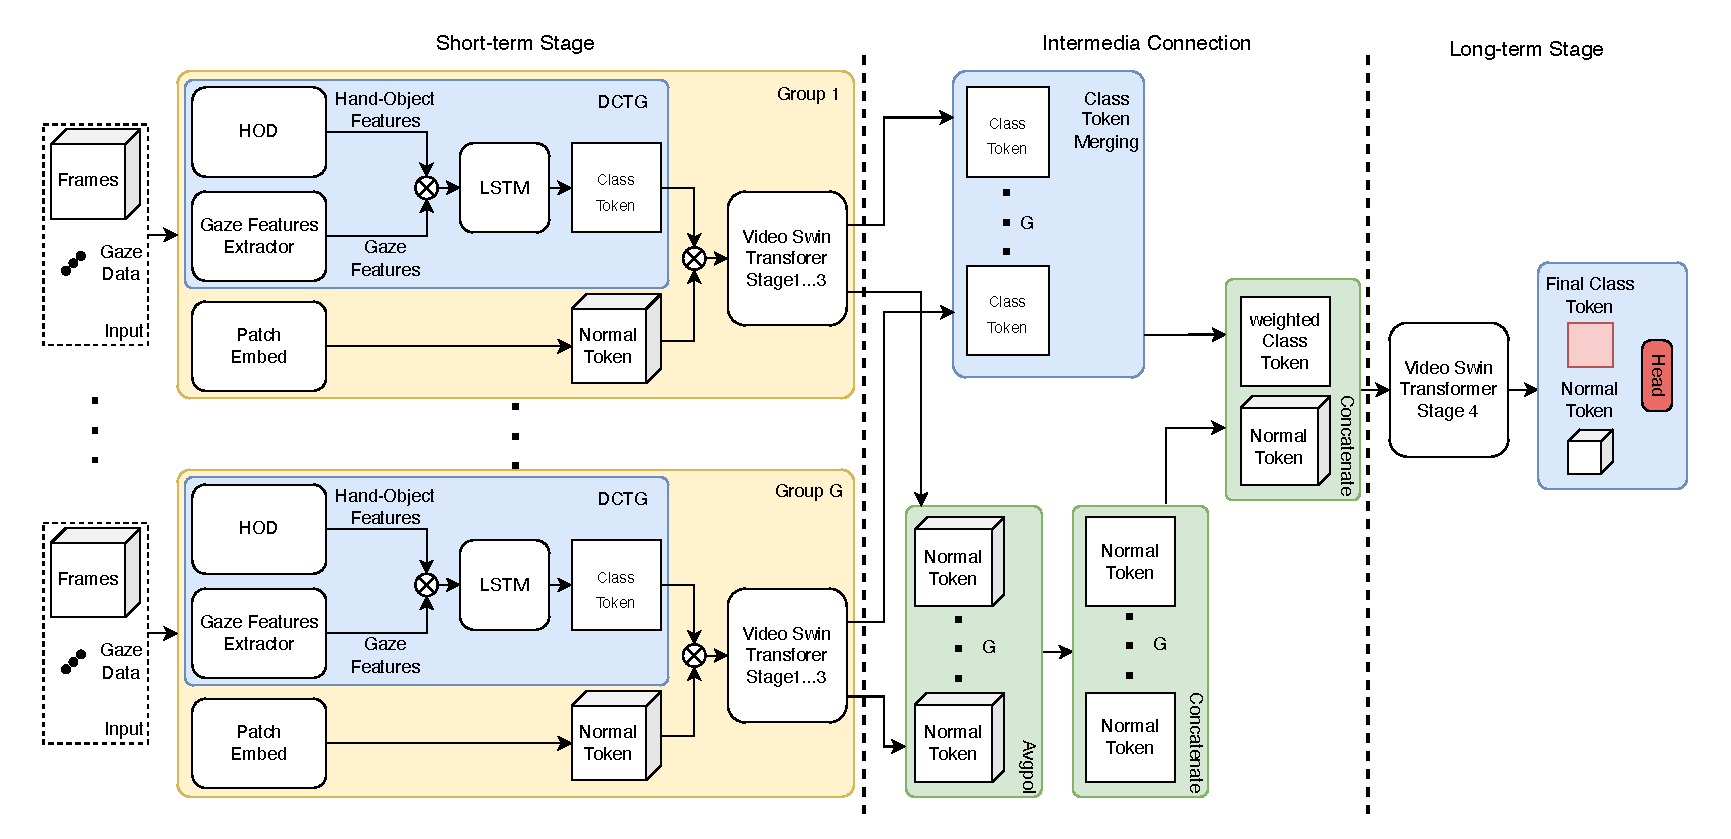
\includegraphics[width=\paperwidth]{graphics/structure.pdf}
    }
    \caption{Overall architecture of the Gaze-Enhanced EgoViT.}
    \label{fig:overall_architecture}
\end{figure}

A Video Transformer commonly converts the input video frames into a sequence of feature vectors. Thus, the input frames can be denoted as the vector $I \in \mathbb{R}^{T_{sampled} \times H\times W\times C}$, where $T_{sampled}$ is the number of frames sampled from the video, $H$ and $W$ are the height and width of the frame, and $C$ is the number of channels. The proposed model includes an additional input of gaze points vector $J \in \mathbb{R}^{T_{sampled} \times 2}$ representing the coordinates $(x, y)$ of the gaze points in the $T_{sampled}$ frames. 

The $T_{sampled}$ frames and their associated $T_{sampled}$ gaze points data are first split into $G$ groups, uniformly distributed along the temporal dimension. The short-term phase of a video clips is denoted as $I_{g} \in \mathbb{R}^{T \times H \times W \times C}$ and the vector of gaze points is denoted as $J_{g} \in \mathbb{R}^{T \times 2}$, where $D = \frac{D_{sampled}}{G}$. The vectors $I_{g}$ and $J_{g}$ are then fed into the Gaze-Enhanced \gls{dctg} module to extract the gaze-hand-object features. The function of Gaze-Enhanced \gls{dctg} will be discussed in detail in section \ref{sec:Gaze-Enhanced DCTG Module}. In parallel, the $I_{g}$ is fed into the PatchEmbedding module in the Video Swin Transformer to extract the features of the video frames. 

The Vector $I_{g}$ is segmented into non-overlapping patches, of size $\mathbb{R}^{P_T \times P_H \times P_W \times C}$. These patches are projected in a flatte layer into sequence data of $\mathbb{R}^{N_P \times (P_T \times P_H \times P_W \times C)}$, where $N_P = T_P \times H_P \times W_P = \frac{T}{P_T} \times \frac{H}{P_H} \times \frac{W}{P_W}$. A liner layer uses a matrix of size $\mathbb{R}^{(P_T \times P_H \times P_W \times C) \times D}$ to project the sequence data into a lower dimension $D$. The embedded vector is denoted as $X_P \in \mathbb{R}^{N_P \times D}$. The output of the Gaze-Enhanced \gls{dctg} module is treated as the class token $x_{cls}$ with the shape $\mathbb{R}^{1 \times D}$, and is concatenated with the sequence data $X_P$ to form the input of the Video Swin Transformer. The Combination of $x_{cls}$ and $X_P$ is performed along the temporal dimension, positioning the class token as the first vector in this dimension. The sequence data $X_P$ is defined as normal token in this model. Therefore, the input to the transformer is defined as:
\begin{equation}
    x= [x_{cls}, X_P] \in \mathbb{R}^{(N_P + 1) \times D}
    \label{eq:input_transformer}
\end{equation}
The class token is designed to leverage the information exchange capabilities of the 3D Shifted Window Self-Attention mechanism in Video Swin Transformer, which facilitates the sharing of information between the class token and the normal token.

The Video Swin Transformer is modified to build the short-term, intermediate and long-term architecture. It is divided in two parts: the PatchEmbedding layers and stage 1 to stage 3 are in the short-term stage, which is responsible for extracting local temporal information. The stage 4 is in the long-term stage, which is responsible for extracting global temporal information. Between the two parts of the Video Swin Transformer, the Dynamic Merging module is used to merge the output of the short-term stage. It calculates the score $\alpha$ of short-term class token for each group. Then, all scores are summed and normalized to obtain the total score $\alpha_{total}$. A weighted class token is then calculated from $\alpha_{total}$ and the class tokens $x^{cls}_g$ of each group. In this module, the weights are assigned, and the class tokens are aggregated based on the short-term actions. The Dynamic Merging module is discussed in detail in section \ref{sec:Dynamic Merging Module}.

The input of long-term stage is the concatenation of the weighted class token $x^{cls}_{st}$ and the normal token $X^{P}_{st}$, where the subscript "st" for short-term. Therefore, the input of the long-term stage is defined as:
\begin{equation}
    x_{lt} = [x^{cls}_{st}, X^{P}_{st}] \in \mathbb{R}^{(N_P + 1) \times D_{st3}}
    \label{eq:input_long_term}
\end{equation}
Where $D_{st}$ is the dimension of the output of the stage3 in Video Swin Transformer and the subscript "lt" denotes for long-term. 

The $x_{lt}$ is fed into the stage 4 of Video Swin Transformer to extract the global temporal information. The final score of the action prediction is calculated from the Head, which computes the score of each action class. The action class with the highest score is selected as the final prediction.
% \begin{landscape}
%     \centering
%     \begin{figure}
%         \centering
%         % 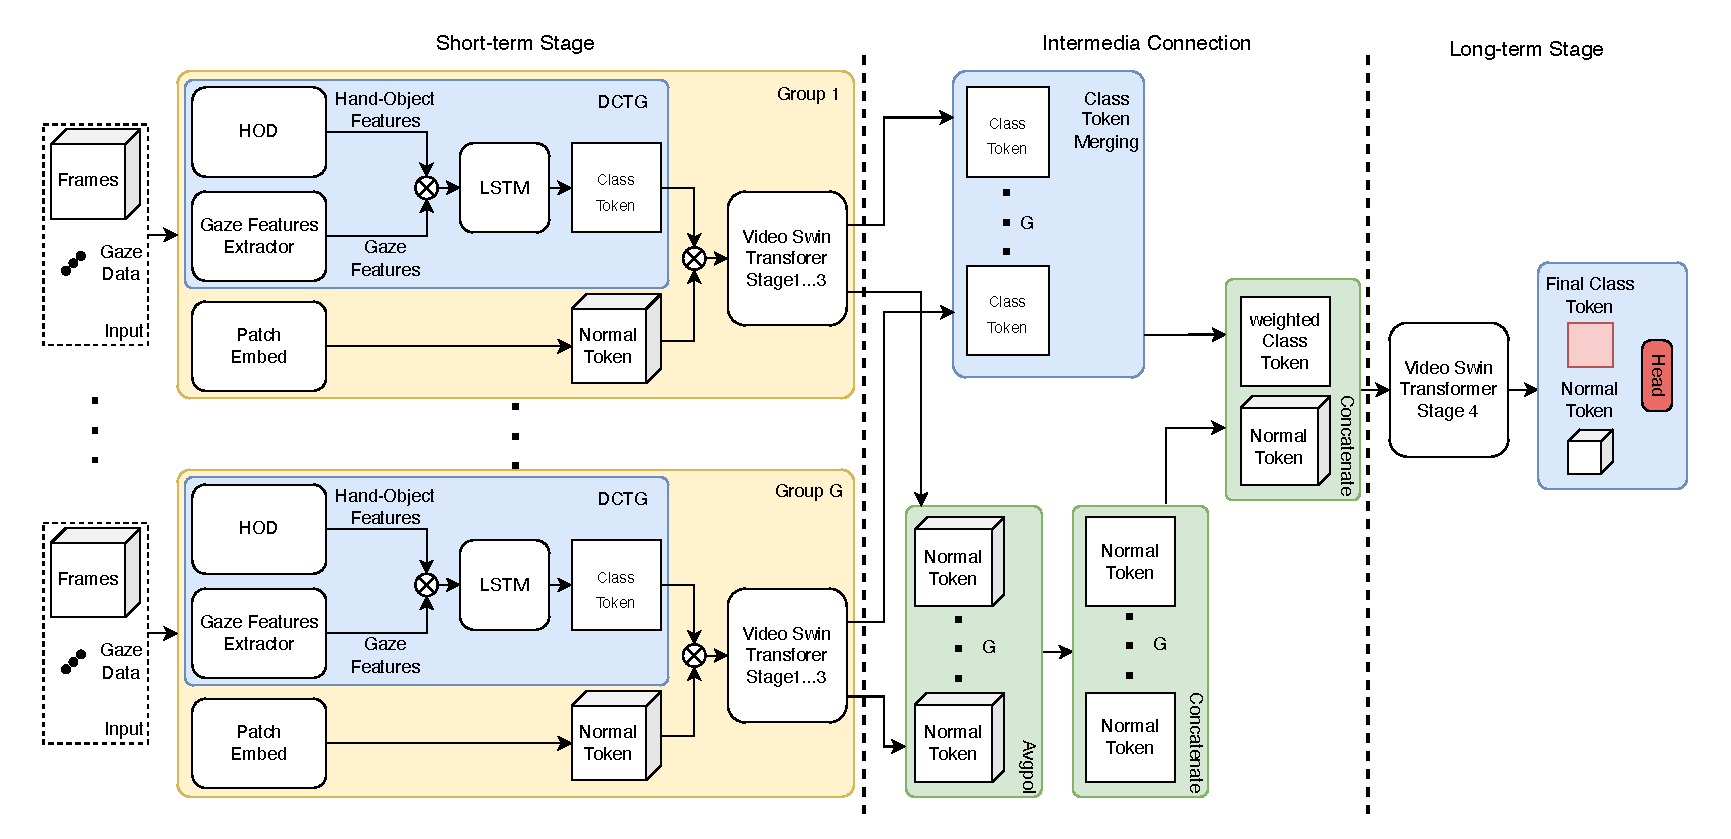
\includegraphics[width=\textwidth]{graphics/structure.pdf}
%         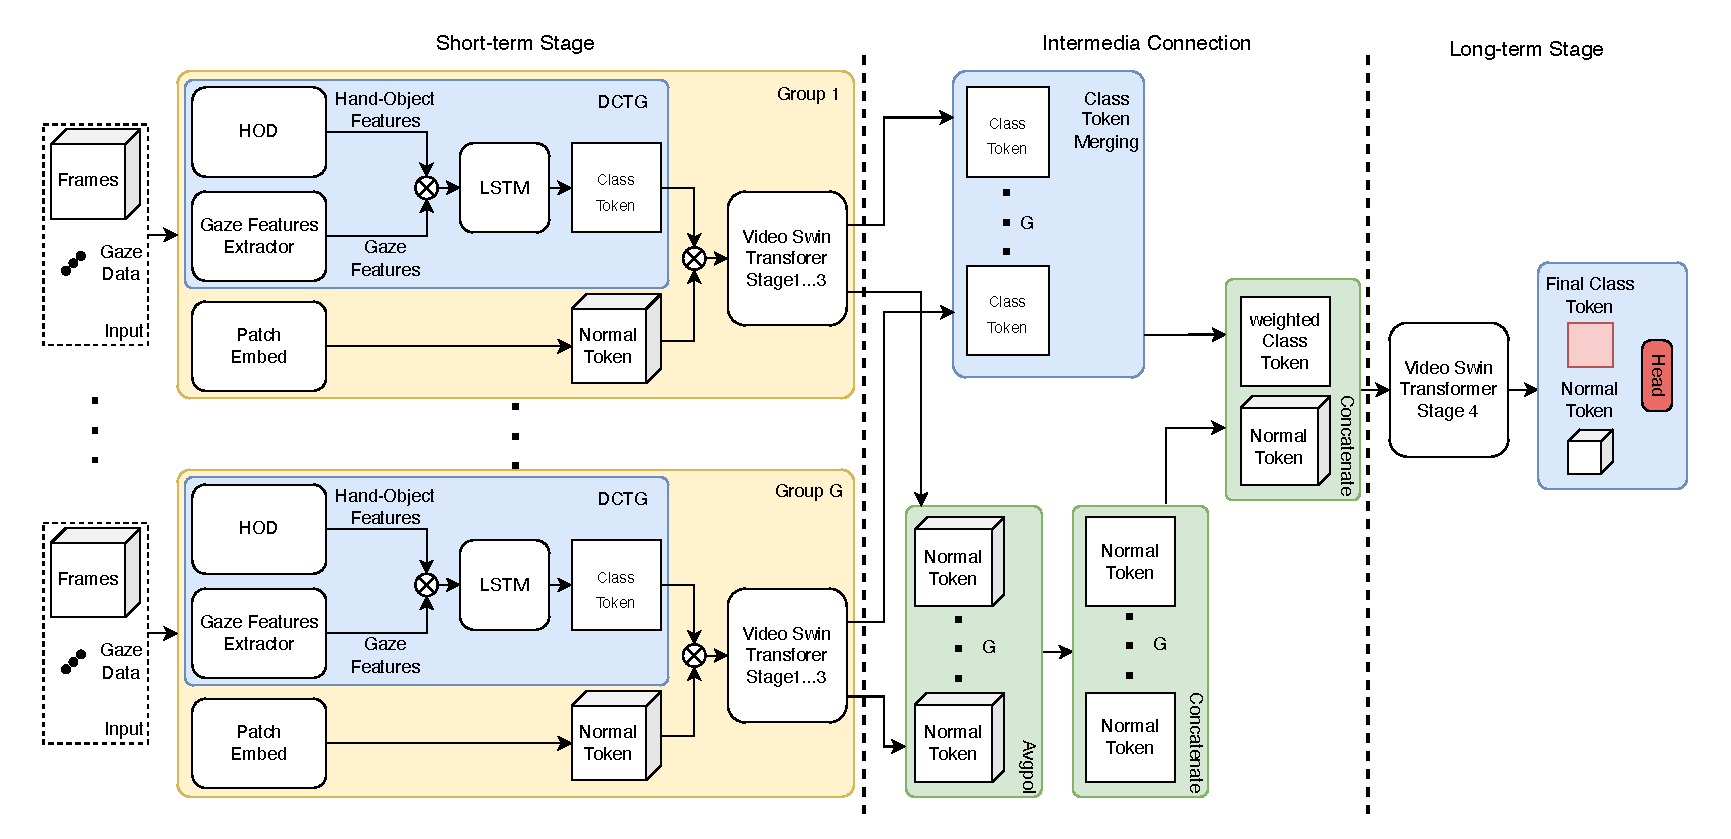
\includegraphics[width=\paperwidth]{graphics/structure.pdf}
%         \caption{The original EgoViT architecture.}
%         \label{fig:ego_vit}
%     \end{figure}
% \end{landscape}

\section{The Gaze-Enhanced DCTG Module}
\label{sec:Gaze-Enhanced DCTG Module}
To integrate gaze information, the Gaze-Enhanced \gls{dctg} module was developed. This module is a key component of the proposed model, responsible for extracting gaze features from the given gaze points and merging them with hand-object features. Finally, a class token is generated from the gaze-hand-object features and fed into subsequent layers. The module consists of three submodules: the Gaze Feature Extractor, the Hand-Object Feature Extractor, and the \gls{lstm} module. The structure of the Gaze-Enhanced \gls{dctg} module is shown in Figure \ref{fig:gaze_dctg}.
\begin{figure}
    \centering
    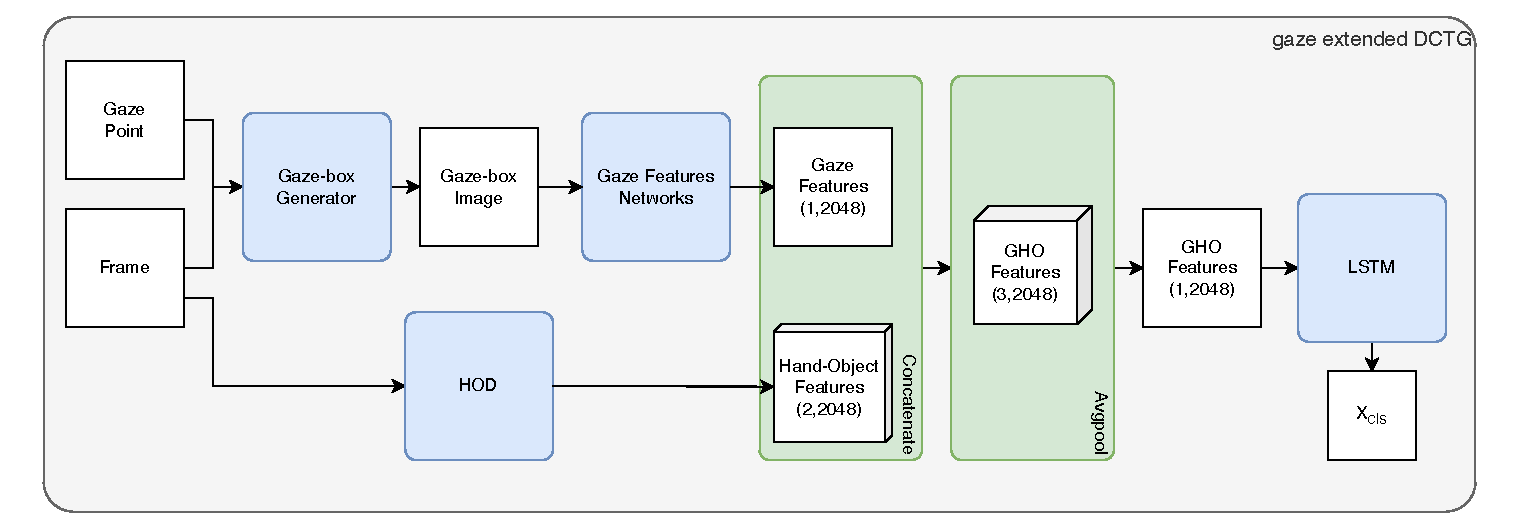
\includegraphics[width=\textwidth]{graphics/dctg.pdf}
    \caption{The data pipeline of the Gaze-Enhanced DCTG module.}
    \label{fig:gaze_dctg}
\end{figure}

The Gaze Feature Extractor is responsible for extracting the gaze features from the given gaze points and frames. The gaze points and frames are first fed into the Gaze-Box Generator. The gaze-box represents the region of the gaze area in the frame, with the gaze point being the center of the gaze region. A square box of size $35 \times 35$ is generated. Based on the gaze-box, a gaze image is cropped from the frame. The gaze image is then fed into the Gaze Feature Networks to extract the gaze features. The $T$ frames and their associated gaze points are sent to the Gaze-Enhanced \gls{dctg}, and the input of the Gaze Feature Networks can be denoted as $I^{gb} \in \mathbb{R}^{T \times 35 \times 35 \times C}$,  where "gb" stands for gaze-box.

The Gaze Feature Networks is a convolutional neural network, as shown in Figure \ref{fig:gaze_feature_networks}. The network consists of three convolutional blocks, each containing a convolutional layer, a batch normalization layer, a ReLU activation layer, and a max-pooling layer.  At the end, the gaze features pass through a flatten layer and a linear layer to generate the output in $D$-dimensions. The output of the Gaze Feature Networks is denoted as $I^{gaze} \in \mathbb{R}^{T \times D}$, where $D$ is the dimension of the gaze features.

\begin{figure}
    \centering
    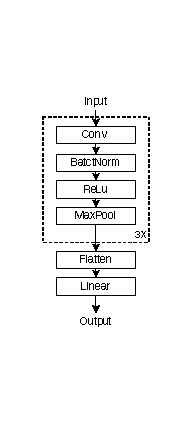
\includegraphics[width=0.5\textwidth]{graphics/gaze_feature_networks.pdf}
    \caption{The structure of the Gaze Feature Networks.}
    \label{fig:gaze_feature_networks}
\end{figure}

A modified \acrlong{hod} module \cite{shan_understanding_2020} is applied offline in this thesis. The \gls{hod} is a pre-trained hand-object detector based on Faster-RCNN networks \cite{ren_faster_2016}. It is designed to detect and classify hands and the objects they interact with in videos. The output consists of the bounding boxes of the hands and objects, as well as their class labels. The code of \gls{hod} is modified to also provide the features of the hands and objects.

Let $I \in \mathbb{R}^{T \times H \times W \times C}$ be the input frames. The \gls{hod} predicts bounding boxes $BB$ for hands and objects,  and a feature map $I^{base}$ is generated by the base part of \gls{hod}. The bounding box predictions are overlapped and, according to the credibility ranking, the top-M hand and top-M object detections with confidence scores $\theta > 0.5$ are chosen. The feature maps, along with the detections, are fed into the “RoIAlign” layers and the “top feature refine” module to generate 2048-dimensional vectors for each detected hand and object.

The hand-object features are denoted as $F^{HO} \in \mathbb{R}^{T \times 2M \times 2048}$, where $2M$ represents the $M$ hand (including left and right) features and $M$ object features. Average pooling is then applied to the $M$ hand features and $M$ object features to generate the final hand-object features, denoted as $I^{HO} \in \mathbb{R}^{T \times 2 \times 2048}$. The hand-object feature extraction process in the Gaze-Enhanced \gls{dctg} module can be described by the following equation:
\begin{equation}
    \begin{aligned}
        &cls_{t}, BB_t = HOD(I_t, \theta_t), \quad \text{for } t \in [1, T] \\[12pt]
        &I_t^{\text{base}} = HOD_{\text{base}}(I_t) \in \mathbb{R}^{1024 \times H^b \times W^b}, \\[12pt]
        &I_t^{\text{align}} = \text{ROIAlign}(I_t^{\text{base}}, BB_t) \in \mathbb{R}^{2M \times 1024 \times H^a \times W^a}, \\[12pt]
        &I_t^{HO} = HOD_{\text{top}}(I_t^{\text{align}}) \in \mathbb{R}^{2M \times 2048}, \\[12pt]
        &F_t^{HO} = \text{AvgPool}(I_t^{HO}) \in \mathbb{R}^{2 \times 2048}, \\[12pt]
        &F^{HO} = [F_1^{HO}, \ldots, F_T^{HO}]  \in \mathbb{R}^{T \times 2 \times 2048}
    \end{aligned}
    \label{eq:hand_object_feature}
\end{equation}
where $I_t$ is the $t$-th frame along temporal axis, $cls_t$ are the class labels of the hands and objects, which are not needed in this thesis. $H^b$ and $W^b$ are the height and width of the feature maps $I_t^{\text{base}}$, $H^a$ and $W^a$ are the height and width of the feature maps $I_t^{\text{align}}$. $M$ is the number of hands and objects detected in each frame.

The extracted gaze features $F^{G} \in \mathbb{R}^{T \times 2 \times 2048}$ and hand-object features $F^{HO} \in \mathbb{R}^{T \times 1 \times 2048}$ are concatenated. Thus, the gaze-hand-object features are denoted as $F^{GHO} \in \mathbb{R}^{T \times 3 \times 2048}$.  The mean value of these three types of features is then calculated as:
\begin{equation}
    \begin{aligned}
        &F^{GHO} = [F^{G}, F^{HO}] \in \mathbb{R}^{T \times 3 \times 2048}, \\[12pt]
        &F^{GHO}_{t} = \frac{1}{3} \sum_{t=1}^{3} F^{GHO}_{t,i}, \quad \text{for } t \in [1, T], \quad i \in [1, 3]
    \end{aligned}
    \label{eq:mean_feature}
\end{equation}
The final gaze-hand-object features are denoted as $F^{GHO} \in \mathbb{R}^{T \times 2048}$. According to \cite{pan_egovit_2023}, applying the \gls{lstm} achievs better performence in aggregating knowledge from the temporal dimension. Therefore, the \gls{lstm} module is applied to generate the class token $x_{cls} \in \mathbb{R}^{T \times D}$ from the gaze-hand-object features $F^{GHO}$. The gaze-hand-object features is projected from 2048-dimensional features to $D$-dimensional features. The \gls{lstm} provided in the pytorch liberary is used in this thesis. The last state of the output of the \gls{lstm} is defined as the class token $x_{cls}$. The procedure for generating the class token can be described as follows:
\begin{equation}
    \begin{aligned}
        &F^{GHO'} = \text{LSTM}([F^{GHO}_1,\ldots , F^{GHO}_T]) \in \mathbb{R}^{T \times D}, \\[12pt]
        &x_{cls} = F^{GHO'}[-1] \in \mathbb{R}^{D}
    \end{aligned}
    \label{eq:class_token}
\end{equation}
where $F^{GHO'}$ is the output of the \gls{lstm} module, and $F^{GHO'}[-1]$ is the last state of the output along the temporal axis.

\section{Integration of Video Swin Transformer}
\label{sec:Integration of Video Swin Transformer}
The Video Swin Transformer is used as the backbone in both the short-term and long-term stages, separated by the Dynamic Merging module. The Video Swin Transformer is modified to fit the architecture of the Gaze-Enhanced EgoViT by dividing it into two parts. The PatchEmbedding layers and stages 1 to 3 are in the short-term stage, responsible for extracting local temporal information. Stage 4 is in the long-term stage, responsible for extracting global temporal information. The configuration of the Video Swin Transformer follows the Swin-B model in \cite{liu_video_2021}.

The structure of the Video Swin Transformer in the short-term stage is shown in Figure \ref{fig:video_swin_transformer}. The 3D local window is defined as $WI \in \mathbb{R}^{WI_T \times WI_H \times WI_W}$. The patches are denoted as $X^P \in \mathbb{R}^{T_P \times H_P \times W_P \times D}$, where $T_{WI} = \frac{T_P}{WI_T}$, $H_{WI} = \frac{H_P}{WI_H}$, and $W_{WI} = \frac{W_P}{WI_W}$. There are a total of $N_{WI} = T_{WI} \times H_{WI} \times W_{WI}$ windows. Unlike a classic vision transformer, the Video Swin Transformer does not use the class token as the first token in the sequence. Instead, the normal token from 3D shifted windows is used to aggregate information. Therefore, the dimension of the class token in the Gaze-Enhanced EgoViT is expanded to assign the same class token to all 3D windows. After the assignment, each 3D window has a class token and updates it independently.
\begin{figure}
    \centering
    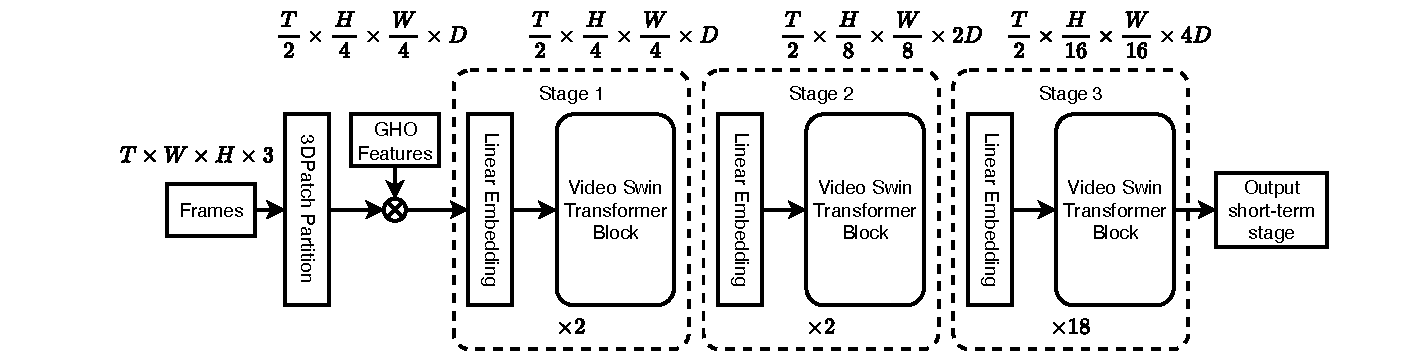
\includegraphics[width=\textwidth]{graphics/vst_st.pdf}
    \caption{The structure and the data pipeline of the short-term stage.}
    \label{fig:video_swin_transformer}
\end{figure}

The input to stage 1 is denoted as:
\begin{equation}
    \begin{aligned}
    &I_{WI,i} = [x_{cls,i}, x_{WI,i}] \quad i \in [1, N_{WI}], \\[12pt]
    &I_{WI,i} \in \mathbb{R}^{((1 + WI_T) \times WI_H \times WI_W) \times D}
    \end{aligned}
\end{equation}
where $i$ denotes the $i^{th}$ window and $x_{WI,i}$ is the normal token of the $i^{th}$ window.

The operation of the dynamic class token in a transformer block is expressed in the following equation:
\begin{equation}
    \begin{aligned}
        \hat{I}_{WI,i}^l &= \text{W-MSA}(\text{LN}(I_{WI,i}^{l-1})) + I_{WI,i}^{l-1}, \\[10pt]
        I_{WI,i}^l &= \text{MLP}(\text{LN}(\hat{I}_{WI,i}^l)) + \hat{I}_{WI,i}^l, \\[10pt]
        \hat{I}_{WI,i}^{l+1} &= \text{SW-MSA}(\text{LN}(I_{WI,i}^l)) + I_{WI,i}^l, \\[10pt]
        I_{WI,i}^{l+1} &= \text{MLP}(\text{LN}(\hat{I}_{WI,i}^{l+1})) + \hat{I}_{WI,i}^{l+1},
    \end{aligned}
\end{equation}
Where LN refers to Layer Normalization, (S)W-MSA refers to the (shifted) Windowed Multi-head Self-Attention, and MLP refers to the Multi-Layer Perceptron. $\hat{I}_{WI,i}^{l}$ and $I_{WI,i}^l$ are the output of (S)W-MSA and MLP in the $l^{th}$ block, respectively. 

The class tokens are attached to the first position in the temporal dimension of the 3D windows.  This produces a hierarchical representation similar to the Video Swin Transformer. The class token neighborhoods within a $2 \times 2$ spatial space are concatenated, which downsamples the spatial dimension by a factor of 2 and increases the $D$-dimensional features by a factor of 4. A linear layer is then applied to project the features to half of their dimension. For example, the output of stage 1 is $\frac{T}{2} \times \frac{H}{4} \times \frac{W}{4} \times D$, then after the Linear Embedding and Transformer Block, the output of the stage 2 becomes $\frac{T}{2} \times \frac{H}{8} \times \frac{W}{8} \times 2D$. Note that downsampling is not applied in the temporal dimension.

\begin{figure}[t]
    \centering
    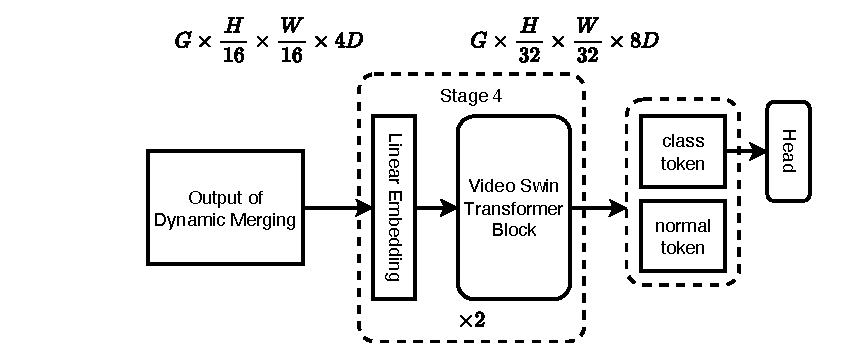
\includegraphics[width=0.9\textwidth]{graphics/vst_lt.pdf}
    \caption{The structure the data pipeline of long-term stage.}
    \label{fig:video_swin_transformer_lt}
\end{figure}

Therefore, the proposed model combines the characteristics of the shifted Window Multi-head Self-Attention and the EgoViT architecture. The shifted Window Multi-head Self-Attention exchanges information in the spatial dimension, while each group in the short-term stage of EgoViT exchanges information in the local temporal dimension. 

The long-term stage consists of the stage 4 of the Video Swin Transformer. The structure and goal of this stage follow the approach in \cite{pan_egovit_2023}, aiming to perceive actions over long durations by exploring the inter-relationships established in the short-term stage. The input tensor $x_{mrg}$ to stage 4 is the concatenation of the weighted class token $x^{cls}_{mrg}$ and the normal token $x^{P}_{mrg}$, which is expressed as:
\begin{equation}
    x_{merge} = [x^{cls}_{mrg}, x^{P}_{mrg}] \in \mathbb{R}^{(1 + G) \times \frac{H}{16} \times \frac{W}{16} \times 4D}
\end{equation}
Figure \ref{fig:video_swin_transformer_lt} shows the structure of the Video Swin Transformer in the long-term stage. After processing in stage 4, the output is separated into two parts: the class token $x^{cls}_{lt} \in \mathbb{R}^{1 \times H^{s4}_{wi} \times W^{s4}_{wi} \times 4D}$ and the normal token $x^{P}_{lt} \in \mathbb{R}^{G \times \frac{H}{32} \times \frac{W}{32} \times 4D}$, where the subscript “lt” denotes the long-term stage, and $H^{s4}_{wi}$ and $W^{s4}_{wi}$ are the height and width of the window in stage 4. Only the class token is fed into the Head to calculate the score for each action class. The Head consists of a sequence of layers, including an Average Pooling layer, a Flatten layer, and a Linear layer, which together transform the class token from 2048-dimensional features to a score between 0 and 1, representing the final score for each action class. 

\section{Dynamic Merging Module}
\label{sec:Dynamic Merging Module}
\begin{figure}[b]
    \centering
    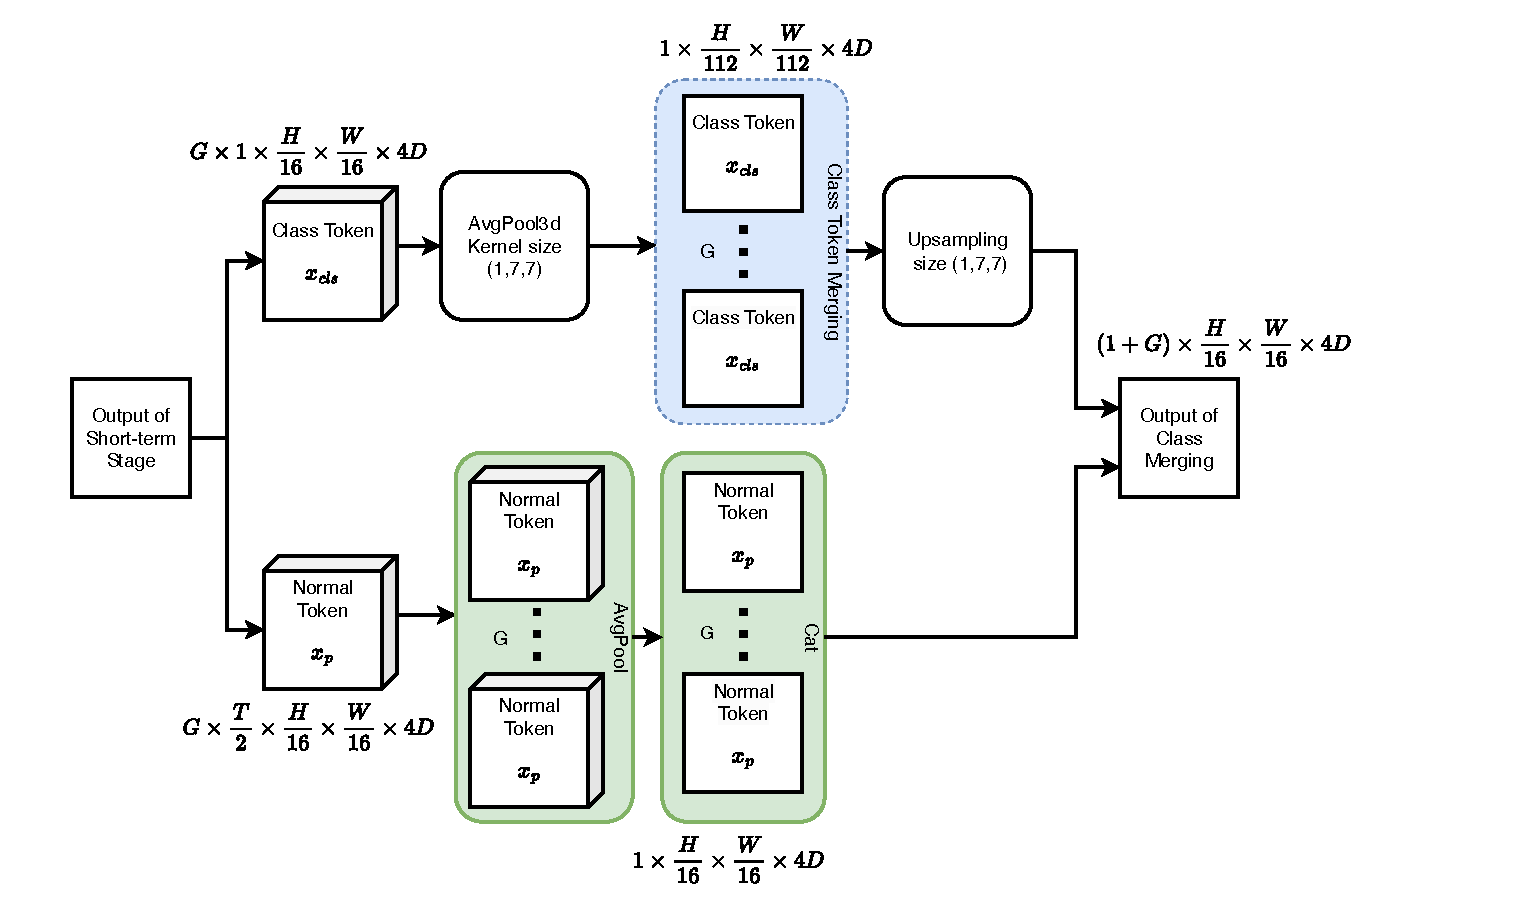
\includegraphics[width=\textwidth]{graphics/dm.pdf}
    \caption{The structure of the Dynamic Merging module.}
    \label{fig:dynamic_merging}
\end{figure}
% \vspace{5mm}
After being processed in the short-term stage, the class token serves as a summary of the short-term actions. The Dynamic Merging module is designed to assign a larger weight to the class tokens representing key short-term actions \cite{pan_egovit_2023}. The structure of the Dynamic Merging module is shown in Figure \ref{fig:dynamic_merging}. The input tensor is $x_{st} \in \mathbb{R}^{G \times (1+\frac{T}{2}) \times \frac{H}{16} \times \frac{W}{16} \times 4D}$. Before merging, the class token $x_{cls}$ and the normal token $x_{P}$ are separated. The class token $x_{cls}$ from each group are fed into an AvgPool3d layer to obtain the class token for each 3D window. According to the window size of the Video Swin Transformer (2, 7, 7), the kernel size of AvgPool3d is set to (1, 7, 7). Then the weighted class token $x^{cls}_{mrg}$ is calculated from the $G$ downsampled class tokens.

The merging algorithm is expressed in Equation \ref{eq:x_cls_s}. First, the dot product between the class tokens of different groups is calculated. The score $\alpha_{g,s,g'}$ is the dot product divided by their l2 norms. The total score $\alpha_{g,s}$ for $x^{cls}_{g,s}$ is calculated by summing the scores along the spatial and group axes. The scores for all class tokens are normalized along the group axis using the softmax operator. The weighted class token $x^{cls}_{mrg}$ for the lont-term stage is then obtained by computing the weighted sum of class tokens along the group axis. Finally, the weighted class token is sent to an upsampling layer with size (1, 7, 7) to match the size of $1 \times \frac{H}{16} \times \frac{W}{16} \times 4D$.

An AvgPool layer is first applied to the $G$ normal tokens $x_{P}$ along the temporal axis, and then the $G$ normal tokens are concatenated to form the normal token with a shape of $G \times \frac{H}{16} \times \frac{W}{16} \times 4D$. At the end of this module, the class token $x^{cls}_{mrg}$ and the normal token $x^{P}_{mrg}$ are concatenated to form the input tensor $x_{lt} \in \mathbb{R}^{(1+G) \times \frac{H}{16} \times \frac{W}{16} \times 4D}$ for the long-term stage. 